\documentclass{report}
\usepackage[utf8]{inputenc}
\usepackage{graphicx}
\usepackage[textheight=700pt]{geometry}


\begin{document}
\renewcommand{\labelitemi}{$\cdot$}

\section*{Qualitätskriterien für Internes und Externes Design}
\subsection*{ISO 9126}
\begin{description}
\item[Functionality / Funktionalität]~\par

Korrektheit, Angemessenheit, Interoperabilität, Ordnungsmäßigkeit, Sicherheit

\item[Reliability / Zuverlässigkeit]~\par

Reife, Fehlertoleranz, Wiederherstellbarkeit

\item[Usability / Benutzbarkeit]~\par

Verständlichkeit, Bedienbarkeit, Erlernbarkeit, Robustheit

\item[Efficiency / Effizienz]~\par

Wirtschaftlichkeit, Zeitverhalten, Verbrauchsverhalten

\item[Maintainability / Wartungsfreundlichkeit]~\par

Analysierbarkeit, Änderbarkeit, Stabilität, Testbarkeit

\item[Portability / Übertragbarkeit]~\par

Anpassbarkeit, Installierbarkeit, Konformität, Austauschbarkeit
\end{description}

\newpage

\section*{Gebrauchstauglichkeit (Benutzbarkeit)}
Kriterien/Facetten für externes Design
\subsection*{ISO 9241-11}
\begin{description}
\item[Effektivität]~\par
Benutzer können ihre
Ziele erreichen
\item[Effizienz]~\par
Benutzer können ihre
Ziele mit angemessenem
Aufwand erreichen
\item[Zufriedenheit]~\par
Benutzer werden nicht in
ihrer Zufriedenheit
beeinträchtigt
\end{description}

\subsection*{Quesenbery}

\begin{description}
\item[Effective]~\par
The completeness and accuracy with
which users achieve their goals.
\item[Efficient]~\par
The speed (with accuracy) in which users
complete their tasks.
\item[Engaging]~\par
How pleasant or satisfying the interface is
to use
\item[Error tolerant]~\par
The ability of the interface to prevent errors
or help users recover from those that occur
\item[Easy to learn]~\par
How well the product supports both initial
orientation and deeper learning
\end{description}

\newpage
\subsection*{Quesenbery lang}
\begin{figure}[ht!]
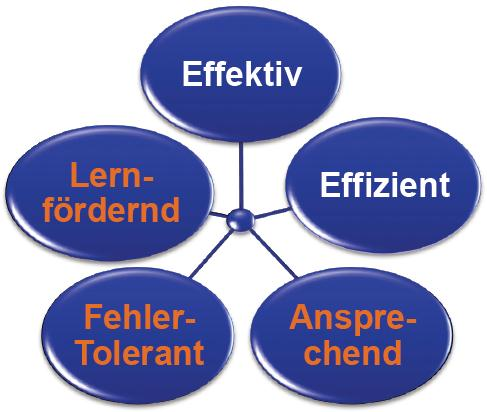
\includegraphics[width=250pt]{overview.png}
\end{figure}

\begin{figure}[ht!]
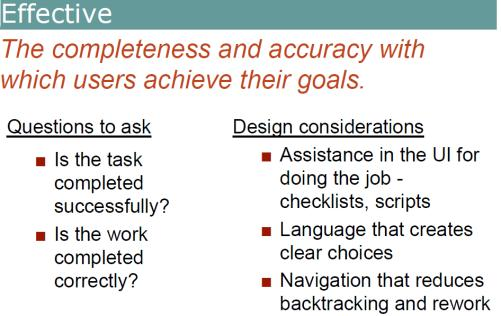
\includegraphics[width=250pt]{effective.png}
\end{figure}

\begin{figure}[ht!]
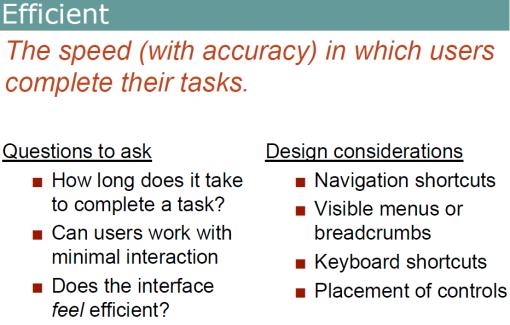
\includegraphics[width=250pt]{efficient.png}
\end{figure}
\newpage
\subsection*{Quesenbery lang}

\begin{figure}[ht!]
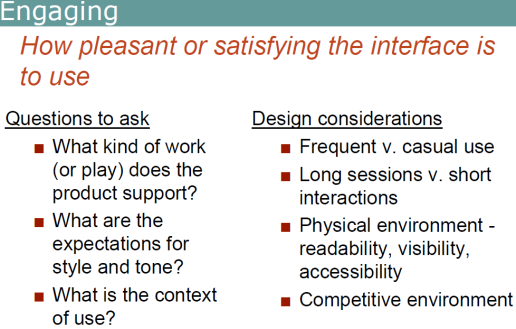
\includegraphics[width=250pt]{engaging.png}
\end{figure}

\begin{figure}[ht!]
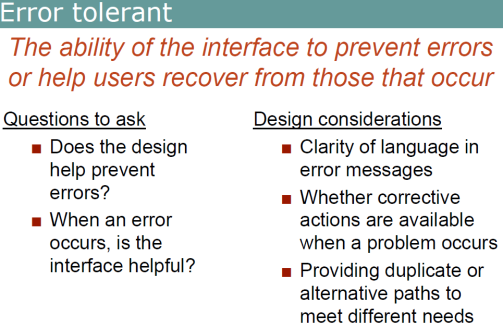
\includegraphics[width=250pt]{errortolerant.png}
\end{figure}

\begin{figure}[ht!]
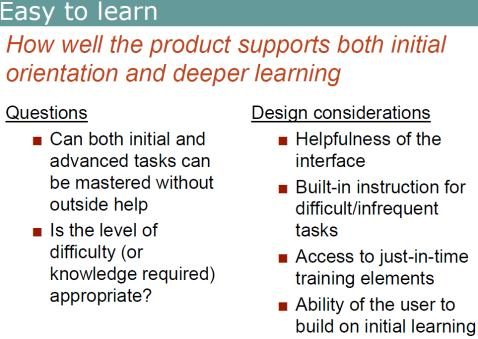
\includegraphics[width=250pt]{easytolearn.png}
\end{figure}

\newpage

\section*{Grundsätze der Dialoggestaltung}
\subsection*{ISO 9241-110}
\begin{description}
\item[Aufgabenangemessenheit]~\par
geeignete Funktionalität, Minimierung unnötiger Interaktionen.\\Beudetet z.B., dass:
\begin{itemize}
    \item Eingabe und Ausgabe dem Benutzer unnötige Arbeitsschritte ersparen (einfaches Sichern und Schließen, sowie erneutes öffnen eines Dokuments)
    \item Der Benutzer mittels automatisierter Abläufe und Voreinstellungen entlastet wird (automatische Startprozeduren, Vorbesetzung mit Standardwerten, Positionieren des Mauscursors usw.)
    \item Keine überflüssige Informationsanzeige oder Hilfestellung gegeben ist.
\end{itemize}

\item[Selbstbeschreibungsfähigkeit]~\par
Verständlichkeit durch Hilfen / Rückmeldungen
\begin{itemize}
\item gilt als erfüllt, wenn für den Anwender jederzeit offensichtlich ist, an welcher Stelle er sich befindet, welche Aktionen wie ausgeführt werden können und Hilfe zum jeweiligen Dialogschritt verfügbar ist.
\end{itemize}

\item[Lernförderlichkeit]~\par
Anleitung des Benutzers, Verwendung geeigneter Metaphern, Ziel: minimale Erlernzeit
\begin{itemize}
\item Ein Dialog ist lernförderlich, wenn er den Benutzer beim Erlernen der Nutzung des interaktiven Systems unterstützt und anleitet.
\end{itemize}

\item[Steuerbarkeit]~\par
Steuerung des Dialogs durch den Benutzer
\begin{itemize}
\item Ein Dialog wird als steuerbar (aus dem niederdeutschen stur "Steuerruder") bezeichnet, wenn der Benutzer in der Lage ist, den Dialogablauf zu starten sowie seine Richtung und Geschwindigkeit zu beeinflussen
\end{itemize}

\item[Erwartungskonformität]~\par
Konsistenz, Anpassung an das Benutzermodell
\begin{itemize}
\item  Anwendungen sind erwartungskonform, wenn sie nach einem einheitlichen Prinzip bedienbar, die Bearbeitungszeiten vorhersehbar, sowie in der Orientierung einheitlich gestaltet sind.
\end{itemize}

\item[Individualisierbarkeit]~\par
\begin{itemize}
\item Anpassbarkeit an Bedürfnisse und Kenntnisse des Benutzers
\end{itemize}

\item[Fehlertoleranz]~\par
Das System reagiert tolerant auf Fehler oder ermöglicht eine leichte Fehlerkorrektur durch den Benutzer
\begin{itemize}
\item Ein Dialog ist fehlertolerant, wenn das beabsichtigte Arbeitsergebnis trotz erkennbar fehlerhafter Eingaben entweder mit keinem oder mit minimalem Korrekturaufwand durch den Benutzer erreicht werden kann
\end{itemize}
\end{description}

\newpage

\subsection*{Schneidermans acht goldene Regeln des Dialog-Design}

\begin{description}
\item[Strebe nach Konsistenz]~\par
Interne und externe Konsistenz
\item[Ermögliche es häufigen Nutzern, Abkürzungen zu benutzen]~\par
Experten und Anfänger unterstützen. Accessibility
\item[Biete informative Rückmeldungen]~\par
Feedback über laufende Funktionen oder den Systemstatus.
\item[Entwerfe abgeschlossene Dialoge]~\par
Klar machen wann eine Funktion/Befehlskette abgeschlossen ist.
\item[Biete einfache Fehlerbehandlung]~\par
Informationen zur Fehlersituation; Auswege.
\item[Erlaube einfache Umkehrung von Aktionen]~\par
Undo-Funktion
\item[Unterstütze interne und lokale Kontrolle]~\par
Benutzer fühlt sich in Kontrolle
\item[Verringere Abfragen des Kurzzeitgedächtnisses]~\par
Anzeigen statt Abfragen

\end{description}

\newpage

\section*{Heuristische Evaluation von GUIs}
\subsection*{Nielsen Kriterien}

\begin{description}
\item[Sichtbarkeit des System-Status]~\par
\begin{itemize}
\item In welchem Bereich befinde ich mich?
\item Was wurde gerade gespeichert? (Name anzeigen oder so)
\item Grund für Disable von Elementen anzeigen
\end{itemize}
\item[Enger Bezug zwischen System und realer Welt]~\par
z.B. Entwickler- \& User-Vokabular sind unterschiedlich
\item[Nutzerkontrolle und Freiheit]~\par
\begin{itemize}
\item Abbrechen (auch mit "falschen" Daten)
\item Speichern (auch mit "falschen" Daten?)
\item Undo
\item Validierung mit Mass
\end{itemize}

\item[Konsistenz \& Konformität mit Standards]~\par
Vermeiden:
\begin{itemize}
\item Sprachgewirr (de/en)
\item Leere Menus
\item Gross- / Kleinschreibung
\end{itemize}

\item[Fehler-Vorbeugung]~\par
\begin{itemize}
\item Disable von sinnlosen Operationen
\item Formate vorgeben (Field Help)
\item Generell: Selektieren statt Eingeben (z.B. Datum)\\
Achtung: Cut \& Paste
\end{itemize}

\item[Besser Sichtbarkeit als Sich-erinnern-Müssen]~\par
\begin{itemize}
\item Menüs statt Kommandos
(ausser für sehr geübte Nutzer; Kombination möglich)
\item Neutippen von Informationen = "Bad Smell"
\end{itemize}

\item[Flexibilität und Nutzungseffizienz]~\par
\begin{itemize}
\item Unterschiedliche Nutzertypen beachten -\textgreater Unterschiedliche Operationsauslösung anbieten (Menüs, Shortcuts, Buttons, Popups, Contextmenu...)
\item Aufgabenorientierte Informationen Anzeigen (Bsp.: Anzahl Schüler als Zusatzinfo in Klassenauswahl-Dropdown)
\end{itemize}

\item[Ästhetik und minimalistischer Aufbau]~\par
\begin{itemize}
\item Benutzer beim Ordnunghalten helfen - gleiches Objekt / Dialog sollte nicht mehrmals geöffnet werden
\end{itemize}

\item[Nutzern helfen, Fehler zu bemerken, zu Diagnostizieren und zu beheben]~\par
\begin{itemize}
\item Undo statt Dialoge
\item Validierung mit Field Help
\end{itemize}
\item[Hilfe und Dokumentation]~\par
Verfügbar \& erreichbar
\end{description}

\newpage

\subsection*{Stone}

\begin{description}
\item[Visibility]~\par Der erste Schritt zum Ziel ist sichtbar
\item[Affordance]~\par (Begreifbarkeit) Aktionsauslösung direkt einsichtig
\item[Feedback]~\par Es ist klar was passiert ist (oder passiert -\textgreater Animation)
\item[Simplicity]~\par Nicht mehr als nötig für die Aufgabe
\item[Structure]~\par Logische und konsistente Organisation
\item[Consistency]~\par Vorhersagbarkeit durch Konsistenz
\item[Tolerance]~\par Fehler vermeiden, Wiederherstellung vereinfachen
\item[Accessibility]~\par Design für alle Personengruppen \& Situationen
\end{description}

\subsection*{Galitz}
Principles of Good Screen Design
\begin{itemize}
\item Reduce visual work
\item Reduce intellectual work
\item Reduce memory work
\item Reduce motor work
\item Minimize or eliminate any
burdens or obstructions
imposed by technology
\end{itemize}

\end{document}
